\section{Sprint 2 - Summary}

At the end of sprint 1, the group had decided on a concept for the flight controller. Our plan was to use the motion capture system Qualisys at KIC as our only source of sensing and do all computations externally. The concept was to have no on-board computation, only a receiver on the quadcopter and a unit to send PWM-signals to the motors. In this way, we could eliminate the need for a on-board chip. 
\\\\
Week one of sprint 2 was the first week of technical work. The first thing we did, was to investigate if it was possible to use Qualisys as our only source of sensing. To investigate if it was possible, the group transferred data between Qualisys and an Arduino by bluetooth. The time between data transfers was measured to be 0,08 seconds (12,5 Hz). In order to achieve stable control the we need a transfer rate of minimum 50 Hz.
\\\\
Additionally, the group built a one-axis test rig (Fig. \ref{fig:firsttestrig}) to see if we could hold a motor-propeller assembly on closed-loop control from Qualisys.

\begin{figure}[h]
        \centering
        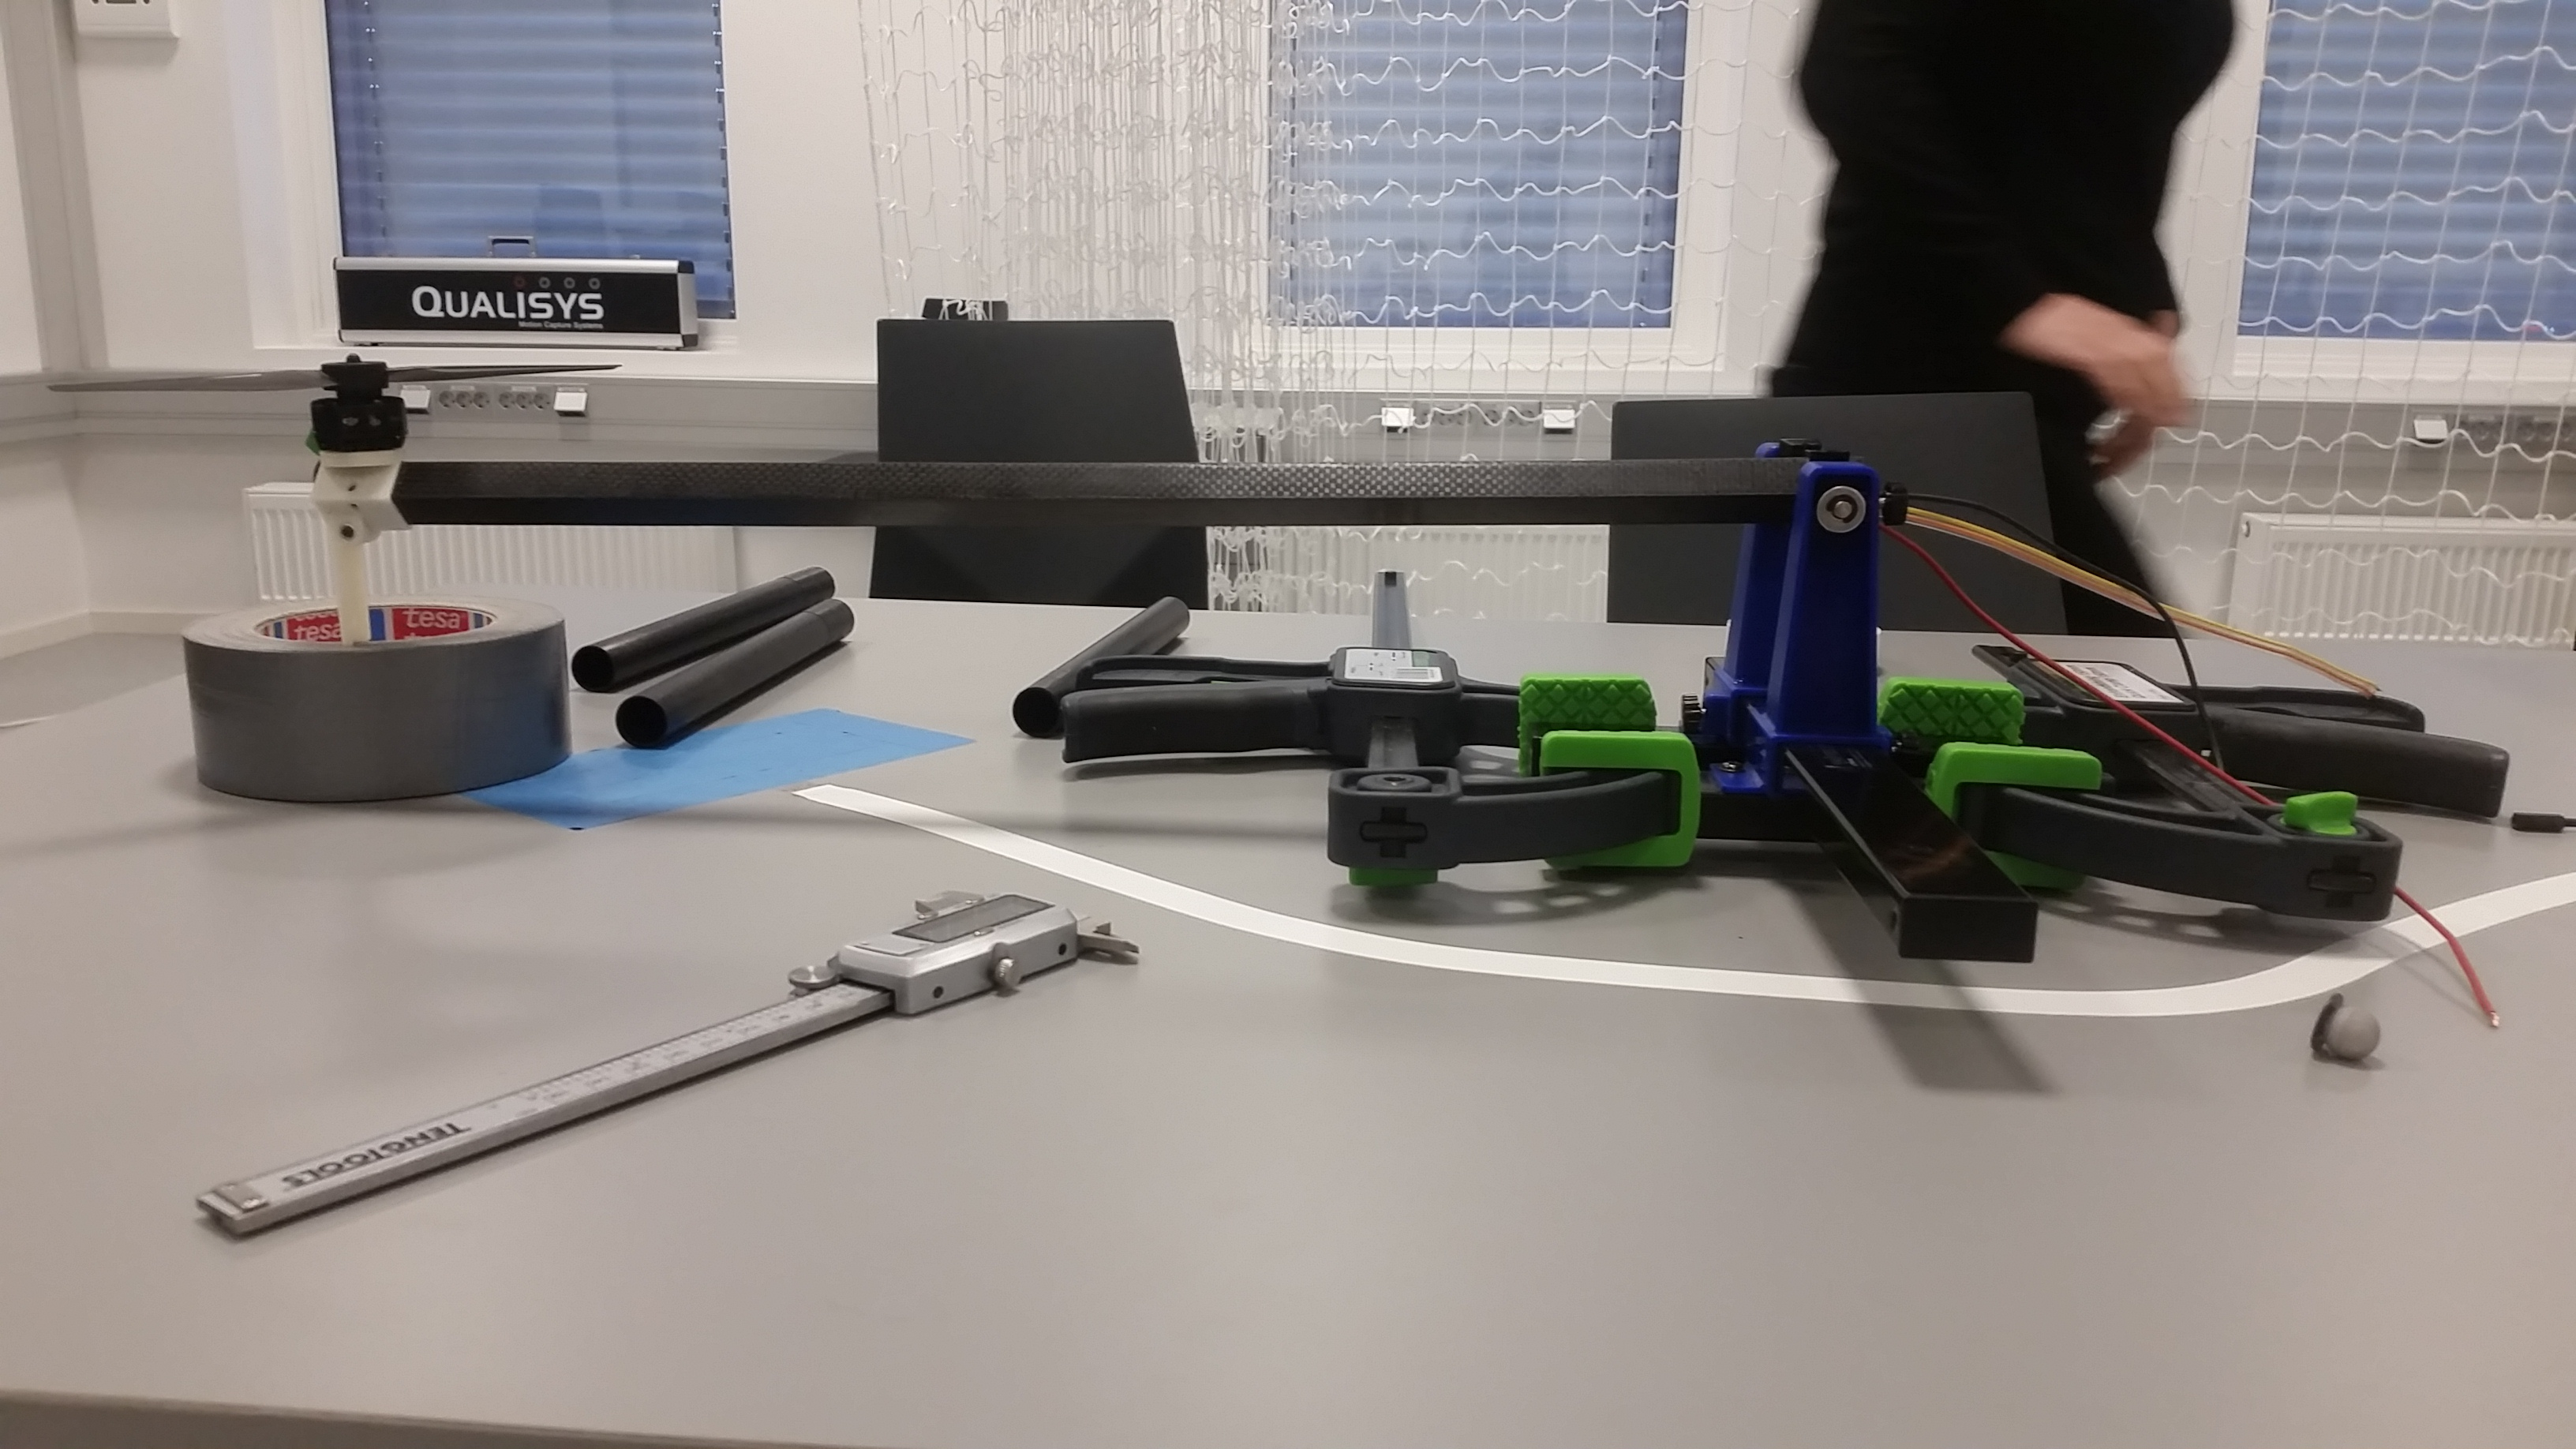
\includegraphics[width = 0.5
        \textwidth]{VAPIQ-PICTURES//TestRig(arm)1}
         \caption{First Test Rig}
         \label{fig:firsttestrig}
    \end{figure}   
\noindent
The team quickly realised that the latency in Qualisys was to great, and concluded that it would be impossible to achieve stable flight with the motion capture system by itself, without on-board computation.
\\
In this sprint, construction of the fixed pitch quadcopter was postponed. The original plan was to use motors which could handle both variable and fixed pitch. If the motors and quadcopters are as equal as possible it will give the best foundation for comparison. Since the motors and mechanisms the group ordered did not work, a new plan and orders had to be placed. 
\\\\
In the meantime, a simple laser-cut fixed pitch quadcopter was assembled with 3DR 880KV AC2836-358 motors borrowed from HSN. This was done in order to test our control algorithm (Fig. \ref{fig:firstfpq}). This was a rapid prototype and only meant for the test bench. In this sprint the preliminary web-page was also published.

\begin{figure}[h]
        \centering
        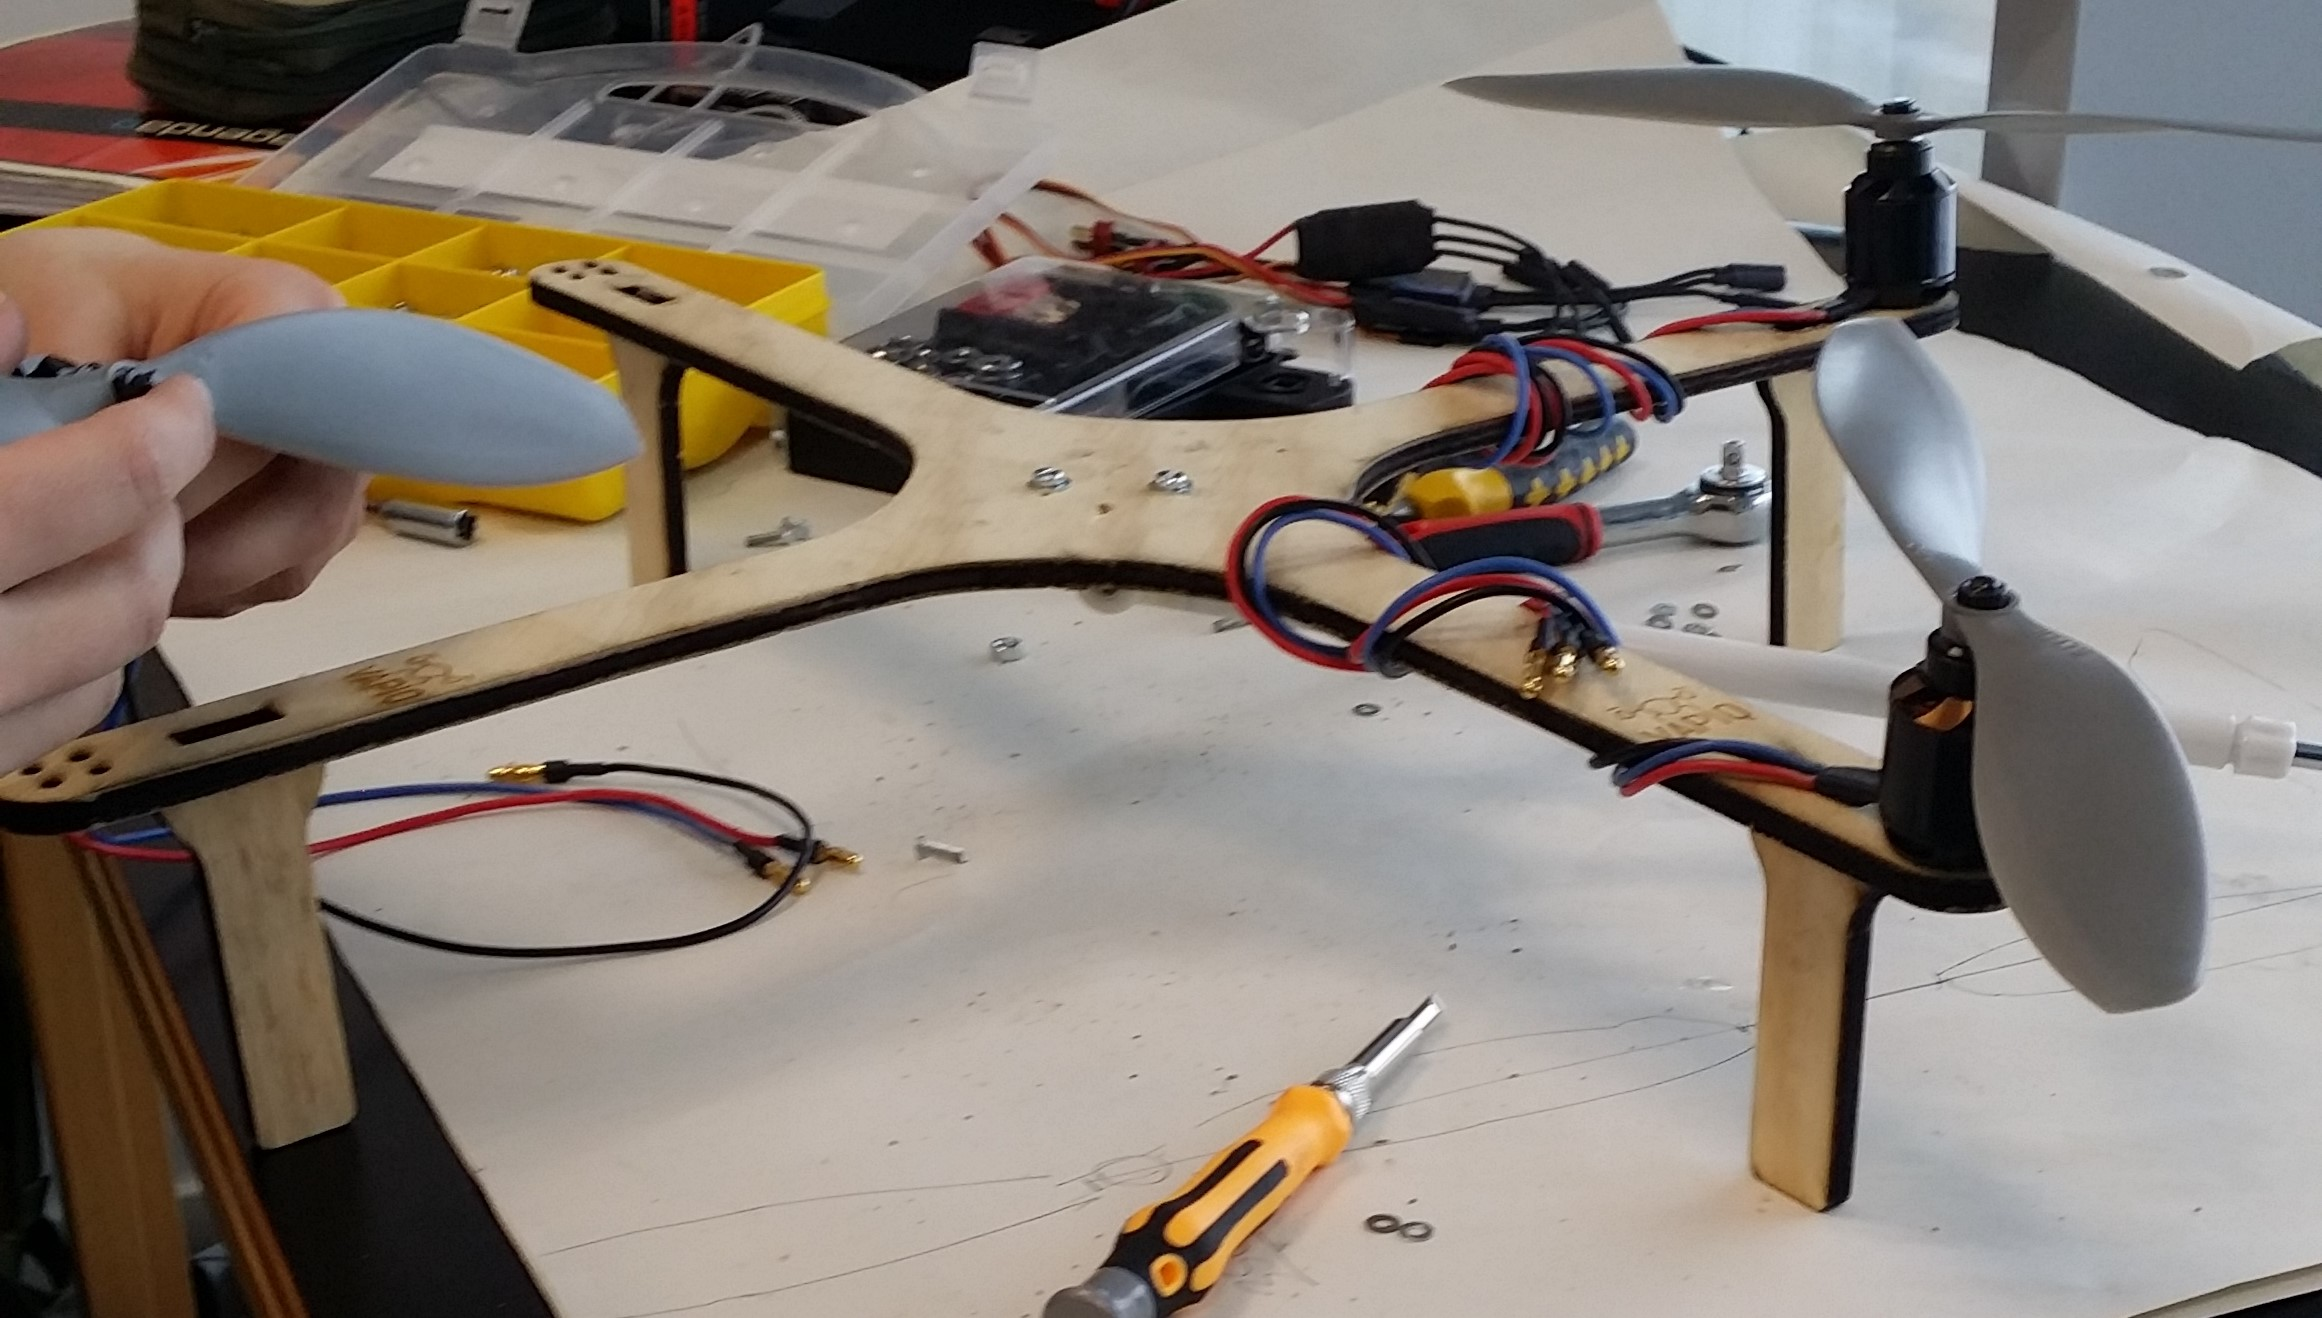
\includegraphics[width = 0.4\textwidth]{VAPIQ-PICTURES//FirstFPQ}
         \caption{First Fixed Pitch Test Copter}
            \label{fig:firstfpq}
    \end{figure}  

\newpage     
\subsection{Completion and Scope Change}

In sprint 2, 79\% of work was completed and the scoop change was 35\%. The scope change was mainly due to the fact that our original plan of using Qualisys as the control system did not work. Therefore we had to reevaluate and find another solution for the flight controller. The group also had plans of making the first fixed pitch quadcopter, but the motors we planned to use did not work. \\
\\
Because of the changes in scope (Fig. \ref{fig:bds2}), some activities in the project plan had to be postponed to sprint 3.
\\\\
Project plan status, sprint 2:

\begin{itemize}
    \item 	Electrical Analysis, \textbf{Postponed}
    \item   Electrical Layout, \textbf{Postponed}
    \item   Electrical Construction, \textbf{Postponed}
    \item   Mathematical Model, Fixed Pitch, \textbf{Postponed}
    \item 	Bluetooth Communication With Arduino, \textbf {Postponed}
    \item 	Mechanical Design Plan, Fixed Pitch, \textbf{Started}
    \item 	Prototype, Fixed Pitch, \textbf{Postponed}
   	\item   Flight Controller Software, \textbf{Started}
    \item 	Publish Web Page, \textbf{Done}
\end{itemize}

\begin{figure}[h]
        \centering
        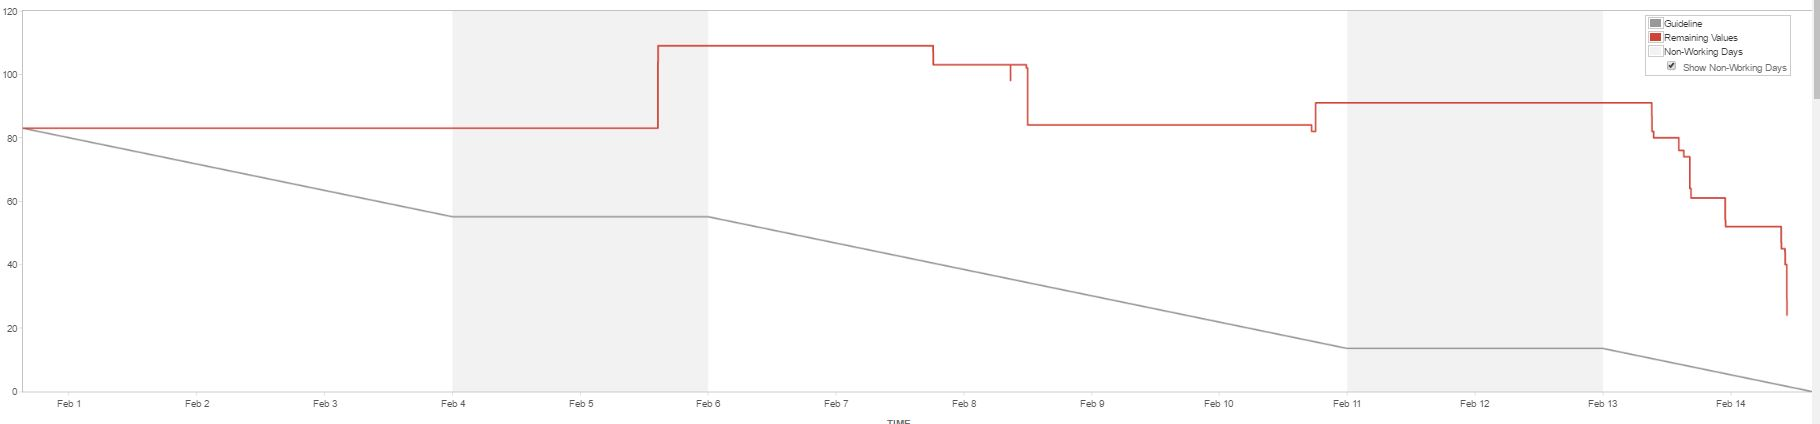
\includegraphics[width = 1
        \textwidth]{VAPIQ-PICTURES//SprintBD2}
         \caption{Sprint 2 - Burndown Chart}
        \label{fig:bds2}
    \end{figure}    

\subsection{Results and Conclusion}

The mechanisms and motors ordered and the plan to use Qualisys to control the quadcopter did not work. A new solution had to be made. There were problems with bluetooth communication because of defect electronics, and have since been resolved. 

